\chapter{视觉定位与三维体积测试与分析}
\label{cha:chap5}
\section{引言}
\label{sec:5.1}
做实验做实验做实验
\section{视觉定位系统测试}
\label{sec:5.2}
\subsection{视觉定位系统实验步骤设计}
\label{sec:5.2.1}
在第二章,本文提出了一种结合二维码的SLAM视觉系统,利用该系统可以估计出带有真实尺度的相机位姿,以及能够得到真实世界坐标系下的
相机位置。本次实验主要利用上述方法在复杂封闭,且无GPS信号的环境下,结合二维码视觉标签进行无人机定位,通过获得到的位置信息信
息进行下一步的飞行控制。本次实验的准备过程主要分为三个步骤,布置场景,生成地图,无人机自主循迹。

首先是场景布置,选择在空旷场地中,布置二维码视觉标签,保证每个二维码的尺度大小完全一致,且二维码之间尽可能等间距布置,场景中的
二维码ID完全独立不同,设计图和实际布置图分别如图~\ref{fig:scene_imagine}和图~\ref{fig:scene_reality}所示。在本次实验中,所原选择的二维码实际大小为0.73m,相邻二维码之间的距
离为4m,整个实验区域面积为400m2(20m*20m)。
\begin{figure}[H] % use float package if you want it here
  \centering
  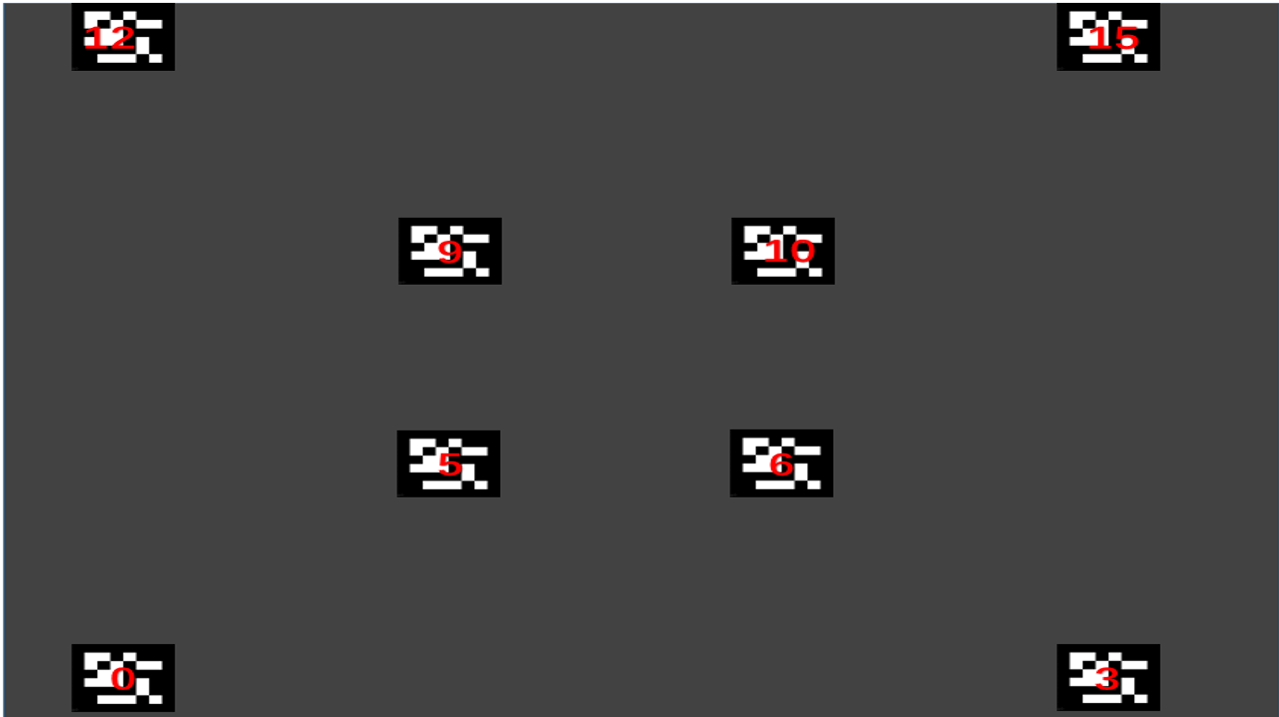
\includegraphics[height=8cm]{scene_imagine.png}
  \caption{ArUco二维码识别结果示意图}
  \label{fig:scene_imagine}
\end{figure}
\begin{figure}[H] % use float package if you want it here
  \centering
  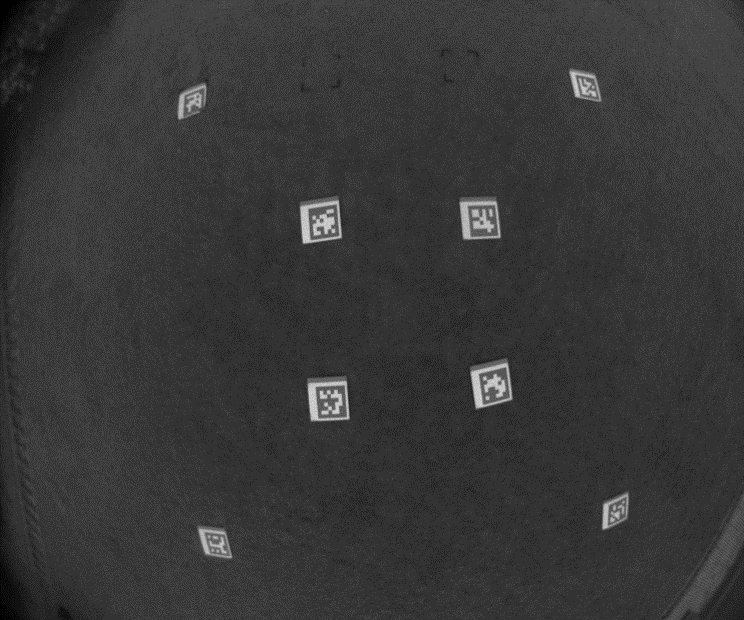
\includegraphics[height=8cm]{scene_reality.png}
  \caption{ArUco二维码识别结果示意图}
  \label{fig:scene_reality}
\end{figure}


